\documentclass[12pt]{article}

\usepackage{amsmath}
\usepackage{enumerate}
\usepackage[margin=5em]{geometry}
\usepackage{multicol}
\usepackage{tikz}

\setlength\parskip{1em}
\setlength\parindent{0em}

\title{Assignment 1}

\author{
	Hendrik Werner s4549775
}

\begin{document}
\maketitle

\section*{9}
\begin{enumerate}[a]
	\item %a
	Every $7^{th}$ number is divisible by 7. There are $999 - 100 = 899$ numbers in the range $[100, 999]$. This means that there are $\lfloor 899 / 7 \rfloor = 128$ numbers divisible by 7 in this range.
	\setcounter{enumi}{3} \item %d
	$\dfrac{3}{4}$ of all natural numbers are not divisible by 4. There are $\lceil \dfrac{3 * 899}{4} \rceil = 675$ numbers in the range $[100, 899]$ which are not divisible by 4.
	\setcounter{enumi}{6} \item %g
	Every $3^{rd}$ number is divisible by 3. There are $\lfloor 899 / 3 \rfloor = 299$ numbers divisible by 3 in the range $[100, 899]$.

	Since we do not want to count the numbers divisible by 4 as well, we subtract the numbers which are divisible by $lcm(3, 4) = 12$. There are $\lfloor 899 / 12 \rfloor = 74$ numbers divisible by 12 in the range $[100, 899]$.

	The final answer are all numbers divisible by 3, without the numbers divisible by 4 as well: $299 - 74 = 225$.
\end{enumerate}

\section*{10}
I assume that 0 is counted as positive for this exercise because there is no solution for $n = 1$ otherwise.

For $n = 1$ there is one solution: $f(1) = 0$.

For $n = 2$ there are four solutions:
\begin{enumerate}
	\item $f(1) = 0, f(2) = 0$
	\item $f(1) = 0, f(2) = 1$
	\item $f(1) = 1, f(2) = 0$
	\item $f(1) = 1, f(2) = 1$
\end{enumerate}

For $n = 3$ there are eight solutions:
\begin{enumerate}
	\item $f(1) = 0, f(2) = 0, f(3) = 0$
	\item $f(1) = 0, f(2) = 0, f(3) = 1$
	\item $f(1) = 0, f(2) = 1, f(3) = 0$
	\item $f(1) = 0, f(2) = 1, f(3) = 1$
	\item $f(1) = 1, f(2) = 0, f(3) = 0$
	\item $f(1) = 1, f(2) = 0, f(3) = 1$
	\item $f(1) = 1, f(2) = 1, f(3) = 0$
	\item $f(1) = 1, f(2) = 1, f(3) = 1$
\end{enumerate}

We can see a pattern emerge: For $n = 0$ there is one function, for $n > 1$, the number of functions is $2^n$.

\section*{11}
We write $\dfrac{n!}{(n - k)!}$ as $n p k$, and $\dfrac{n!}{k!(n - k)!}$ as $n c k$.

\begin{enumerate}[a]
	\item %a
	The photographer chooses a spot for the bride first. There are 6 possible spots for her.

	Next he chooses a permutation (order is important) of 5 other people to fill the remaining spots, from the other 9 people: $9p5 = 15120$.

	Total: $6 * 15120 = 90720$ possibilities.
	\item %b
	The photographer begins by placing the bride first. There are 6 spots for her. After the bride has been placed, there are 5 spots left for the groom.

	Now 8 people remain and we need a permutation of 4 of them: $8p4 = 1680$.

	Total: $6 * 5 * 1680 = 50400$ possibilities.
	\item %c
	The photographer places either the bride or groom in one of 6 spots first. The other one is out for this picture.

	Out of the remaining 8 people, he chooses a permutation of 5: $8p5 = 6720$

	Total: $6 * 6720 = 40320$ possibilities.
\end{enumerate}

\section*{12}
We can show this by providing an example. If we represent each person as a node, and the relations of the persons to each other as edges in the graph, we can rephrase the question as: Can we find a coloring for a fully connected 5-node graph using 2 colors, such that for each color there is no cycle of length 3.

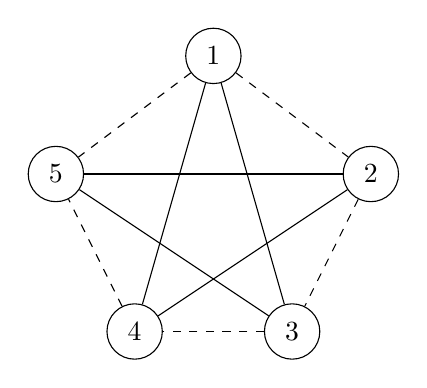
\begin{tikzpicture}[
	c/.style={circle, draw, minimum width=2em}
]
	\node[c] (A) at (0, 1.5) {1};
	\node[c] (B) at (2, 0) {2};
	\node[c] (C) at (1, -2) {3};
	\node[c] (D) at (-1, -2) {4};
	\node[c] (E) at (-2, 0) {5};

	\draw[dashed] (A) -- (B);
	\draw (A) -- (C);
	\draw (A) -- (D);
	\draw[dashed] (A) -- (E);
	\draw[dashed] (B) -- (C);
	\draw (B) -- (D);
	\draw (B) -- (E);
	\draw[dashed] (C) -- (D);
	\draw (C) -- (E);
	\draw[dashed] (D) -- (E);
\end{tikzpicture}

This example shows that we can construct such a graph.

\section*{13}
\begin{enumerate}[a]
	\item %a
	We can prove the existence of such a number with the pigeonhole principle. We make 19 buckets of numbers according to their equivalence class $\mod 19$.

	We take 20 numbers consisting of only 7s: $7, 77, 777, \dots, 77777777777777777777$ and put them into their corresponding bucket. At this point, according to the pigeonhole principle, there is at least one bucket with at least two numbers in it.

	We look for a bucket with 2 numbers and subtract the smaller number from the bigger one. We are left with a number of the form $7 \dots 0 \dots \equiv 0 (\mod 19)$, which has a maximum length of 20 digits.

	\item %b
	\begin{multicols}{2}
	\begin{enumerate}[1]
		\item
		\begin{tabular}{r|l}
			Bucket & Number\\\hline\hline
			7 & 7
		\end{tabular}
		\item
		\begin{tabular}{r|l}
			Bucket & Number\\\hline\hline
			1 & 77\\\hline
			7 & 7
		\end{tabular}
		\item
		\begin{tabular}{r|l}
			Bucket & Number\\\hline\hline
			1 & 77\\\hline
			7 & 7\\\hline
			17 & 777
		\end{tabular}
		\item
		\begin{tabular}{r|l}
			Bucket & Number\\\hline\hline
			1 & 77\\\hline
			6 & 7777\\\hline
			7 & 7\\\hline
			17 & 777
		\end{tabular}
		\item
		\begin{tabular}{r|l}
			Bucket & Number\\\hline\hline
			1 & 77\\\hline
			6 & 7777\\\hline
			7 & 7\\\hline
			10 & 77777\\\hline
			17 & 777
		\end{tabular}
		\item
		\begin{tabular}{r|l}
			Bucket & Number\\\hline\hline
			1 & 77\\\hline
			6 & 7777\\\hline
			7 & 7\\\hline
			10 & 77777\\\hline
			12 & 777777\\\hline
			17 & 777
		\end{tabular}
		\item
		\begin{tabular}{r|l}
			Bucket & Number\\\hline\hline
			1 & 77\\\hline
			6 & 7777\\\hline
			7 & 7\\\hline
			10 & 77777\\\hline
			12 & 777777\\\hline
			13 & 7777777\\\hline
			17 & 777
		\end{tabular}
		\item
		\begin{tabular}{r|l}
			Bucket & Number\\\hline\hline
			1 & 77\\\hline
			4 & 77777777\\\hline
			6 & 7777\\\hline
			7 & 7\\\hline
			10 & 77777\\\hline
			12 & 777777\\\hline
			13 & 7777777\\\hline
			17 & 777
		\end{tabular}
		\item
		\begin{tabular}{r|l}
			Bucket & Number\\\hline\hline
			1 & 77\\\hline
			4 & 77777777\\\hline
			6 & 7777\\\hline
			7 & 7\\\hline
			9 & 777777777\\\hline
			10 & 77777\\\hline
			12 & 777777\\\hline
			13 & 7777777\\\hline
			17 & 777
		\end{tabular}
		\item
		\begin{tabular}{r|l}
			Bucket & Number\\\hline\hline
			1 & 77\\\hline
			2 & 7777777777\\\hline
			4 & 77777777\\\hline
			6 & 7777\\\hline
			7 & 7\\\hline
			9 & 777777777\\\hline
			10 & 77777\\\hline
			12 & 777777\\\hline
			13 & 7777777\\\hline
			17 & 777
		\end{tabular}
		\item
		\begin{tabular}{r|l}
			Bucket & Number\\\hline\hline
			1 & 77\\\hline
			2 & 7777777777\\\hline
			4 & 77777777\\\hline
			6 & 7777\\\hline
			7 & 7\\\hline
			8 & 77777777777\\\hline
			9 & 777777777\\\hline
			10 & 77777\\\hline
			12 & 777777\\\hline
			13 & 7777777\\\hline
			17 & 777
		\end{tabular}
		\item
		\begin{tabular}{r|l}
			Bucket & Number\\\hline\hline
			1 & 77\\\hline
			2 & 7777777777\\\hline
			4 & 77777777\\\hline
			6 & 7777\\\hline
			7 & 7\\\hline
			8 & 77777777777\\\hline
			9 & 777777777\\\hline
			10 & 77777\\\hline
			11 & 777777777777\\\hline
			12 & 777777\\\hline
			13 & 7777777\\\hline
			17 & 777
		\end{tabular}
		\item
		\begin{tabular}{r|l}
			Bucket & Number\\\hline\hline
			1 & 77\\\hline
			2 & 7777777777\\\hline
			3 & 7777777777777\\\hline
			4 & 77777777\\\hline
			6 & 7777\\\hline
			7 & 7\\\hline
			8 & 77777777777\\\hline
			9 & 777777777\\\hline
			10 & 77777\\\hline
			11 & 777777777777\\\hline
			12 & 777777\\\hline
			13 & 7777777\\\hline
			17 & 777
		\end{tabular}
		\item
		\begin{tabular}{r|l}
			Bucket & Number\\\hline\hline
			1 & 77\\\hline
			2 & 7777777777\\\hline
			3 & 7777777777777\\\hline
			4 & 77777777\\\hline
			6 & 7777\\\hline
			7 & 7\\\hline
			8 & 77777777777\\\hline
			9 & 777777777\\\hline
			10 & 77777\\\hline
			11 & 777777777777\\\hline
			12 & 777777\\\hline
			13 & 7777777\\\hline
			17 & 777\\\hline
			18 & 77777777777777
		\end{tabular}
		\item
		\begin{tabular}{r|l}
			Bucket & Number\\\hline\hline
			1 & 77\\\hline
			2 & 7777777777\\\hline
			3 & 7777777777777\\\hline
			4 & 77777777\\\hline
			6 & 7777\\\hline
			7 & 7\\\hline
			8 & 77777777777\\\hline
			9 & 777777777\\\hline
			10 & 77777\\\hline
			11 & 777777777777\\\hline
			12 & 777777\\\hline
			13 & 7777777\\\hline
			16 & 777777777777777\\\hline
			17 & 777\\\hline
			18 & 77777777777777
		\end{tabular}
		\item
		\begin{tabular}{r|l}
			Bucket & Number\\\hline\hline
			1 & 77\\\hline
			2 & 7777777777\\\hline
			3 & 7777777777777\\\hline
			4 & 77777777\\\hline
			6 & 7777\\\hline
			7 & 7\\\hline
			8 & 77777777777\\\hline
			9 & 777777777\\\hline
			10 & 77777\\\hline
			11 & 777777777777\\\hline
			12 & 777777\\\hline
			13 & 7777777\\\hline
			15 & 7777777777777777\\\hline
			16 & 777777777777777\\\hline
			17 & 777\\\hline
			18 & 77777777777777
		\end{tabular}
		\item
		\begin{tabular}{r|l}
			Bucket & Number\\\hline\hline
			1 & 77\\\hline
			2 & 7777777777\\\hline
			3 & 7777777777777\\\hline
			4 & 77777777\\\hline
			5 & 77777777777777777\\\hline
			6 & 7777\\\hline
			7 & 7\\\hline
			8 & 77777777777\\\hline
			9 & 777777777\\\hline
			10 & 77777\\\hline
			11 & 777777777777\\\hline
			12 & 777777\\\hline
			13 & 7777777\\\hline
			15 & 7777777777777777\\\hline
			16 & 777777777777777\\\hline
			17 & 777\\\hline
			18 & 77777777777777
		\end{tabular}
		\item
		\begin{tabular}{r|l}
			Bucket & Number\\\hline\hline
			0 & 777777777777777777\\\hline
			1 & 77\\\hline
			2 & 7777777777\\\hline
			3 & 7777777777777\\\hline
			4 & 77777777\\\hline
			5 & 77777777777777777\\\hline
			6 & 7777\\\hline
			7 & 7\\\hline
			8 & 77777777777\\\hline
			9 & 777777777\\\hline
			10 & 77777\\\hline
			11 & 777777777777\\\hline
			12 & 777777\\\hline
			13 & 7777777\\\hline
			15 & 7777777777777777\\\hline
			16 & 777777777777777\\\hline
			17 & 777\\\hline
			18 & 77777777777777
		\end{tabular}
		\item
		\begin{tabular}{r|l}
			Bucket & Number\\\hline\hline
			0 & 777777777777777777\\\hline
			1 & 77\\\hline
			2 & 7777777777\\\hline
			3 & 7777777777777\\\hline
			4 & 77777777\\\hline
			5 & 77777777777777777\\\hline
			6 & 7777\\\hline
			7 & 7, 7777777777777777777\\\hline
			8 & 77777777777\\\hline
			9 & 777777777\\\hline
			10 & 77777\\\hline
			11 & 777777777777\\\hline
			12 & 777777\\\hline
			13 & 7777777\\\hline
			15 & 7777777777777777\\\hline
			16 & 777777777777777\\\hline
			17 & 777\\\hline
			18 & 77777777777777
		\end{tabular}
	\end{enumerate}
	\end{multicols}

	At this point we have a bucket with 2 numbers in it. If we subtract the smaller number from the bigger one, we get $7777777777777777777 - 7 = 7777777777777777770 \equiv 0 (\mod 19)$.

	Please let me know in the feedback,
	\begin{enumerate}
		\item if there is a better way to to this
		\item if 777777777777777777 would have been a valid example as well, because it consists of 18 7s and 0 0s, and is 0 modulo 19. I am not sure if the numbers are allowed to have 0 0s.
	\end{enumerate}
\end{enumerate}

\end{document}
